  \section{Hardware}
Efter den indledende identifikation og specifikation i design og kravspecifikationen kan implementeringsfasen nu udføres. Hardware implementering af \textit{The Cell Collector} består af enhedstest af hver komponent, med følgende dokumentation. Enhedstestene er lavet i den skrevne rækkefølge og integreret i samme. I dette afsnit vil der være kredsløbsdiagrammer, teori, beregninger og beskrivelser, hvilket er udarbejdet sideløbende med udviklingen af produktet. 
 	
 \subsection{Vægtcelle}
Vægtcellen skal kontrollere om opløsningsbeholderen er tom. Dette afsnit er i tæt knyttet til designdokumentet.

\subsubsection{Enhedstest af vægtcelle }

Efter at diagrammet er fastlagt testes forbindelserne på et \textit{fumlebræt}. Se figur \ref{fig:loadcelltest} for test opstilling.

  \begin{figure}[H]
	\centering
	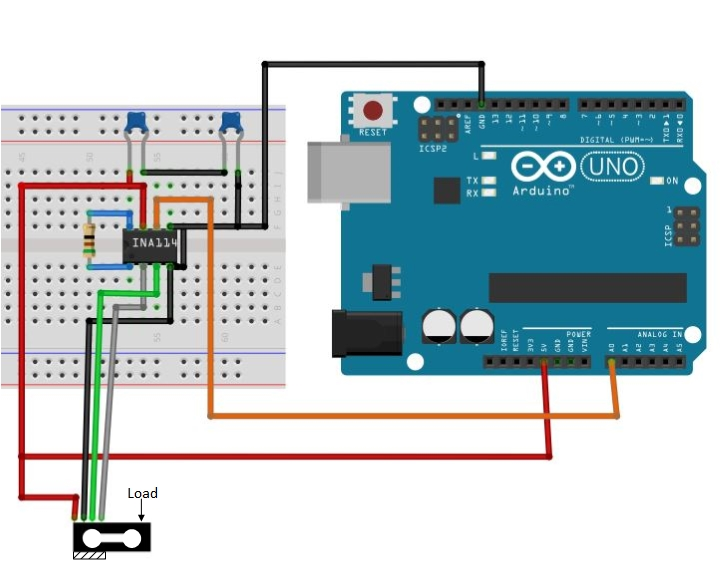
\includegraphics[width=0.9\textwidth]{billeder/Hardware/diagrammer/Drawing1.jpg}
	\caption{Test opstilling for vægtcelle}
	\label{fig:loadcelltest}
\end{figure}
De primære dele af test koden har været  \textit{sensorValue = analogRead(A0);} og \textit{Serial.println(sensorValue);}, hvor inputtet på \textit{A0} er læst i \textit{serial monitor} som vist på figur \ref{fig:loadcell_test} ved langsom tømning af beholderen.

\begin{figure}[H]
	\centering
	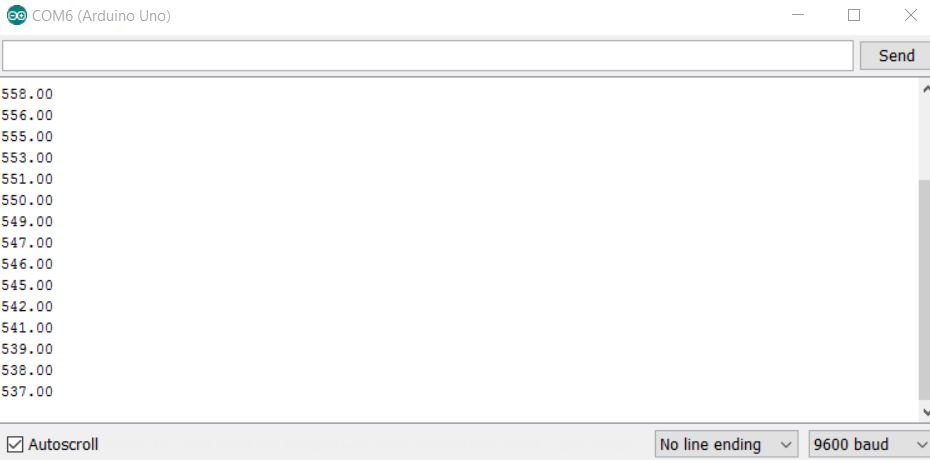
\includegraphics[width=0.9\textwidth]{billeder/Hardware/diagrammer/loadcellunittestbits.JPG}
	\caption{Værdier fra A0 i \textit{serial monitor}}
	\label{fig:loadcell_test}
\end{figure}

 Se bilag \ref{bilag:TKloadcell} for at se hele koden til testen. Til enhedstesten er der brugt et voltmeter til, at måle udgangsspændingen på INA114 for, at se om Arduinoens ADC læste rigtigt. Til at sammenligne med voltmeteret, blev \ref{eq:trintilvolt} brugt til at konvertere ADC'ens bit værdi om til spænding.
 
 \begin{align}
 analogRead(A_0)*\frac{5}{1024}=\text{spænding i volt}
 \label{eq:trintilvolt}
 \end{align}
Testopstilling af vægtcellen ser ud som på \ref{fig:loadcell_mont} med celleopløsningsbeholderen. I softwaren kræves det en kalibrering for at vægtcellen er præcis. Dette er implementeret i afsnit \ref{subsub:softwareloadcell}.
 
 \begin{figure}[H]
	\centering
	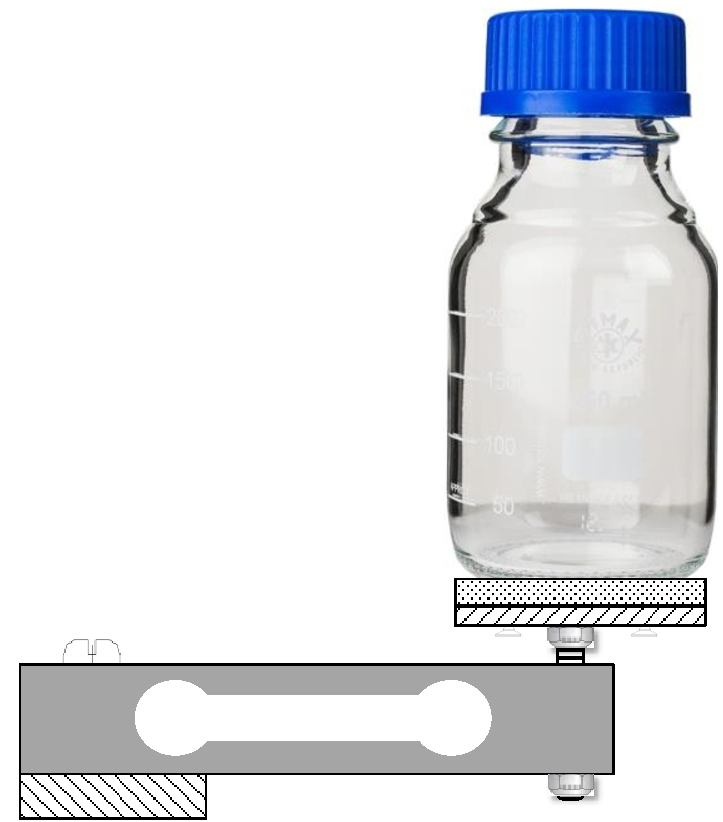
\includegraphics[width=0.5\textwidth]{billeder/Hardware/diagrammer/loadcell_montering.pdf}
	\caption{Illustration af opstilling med vægtcelle og celleopløsningsbeholder}
	\label{fig:loadcell_mont}
\end{figure}

\subsection{Pumpe}
 Pumpen består af en DC motor. Ud fra databladet kan det ses, at den skal bruge 12VDC og 0.3A for at køre. Da Arduinoen langt fra kan levere den nødvendige strøm til at drive motoren, skal der bruges en motordriver med en ekstern strømforsyning.
 

\subsubsection{Enhedstest af motor og motordriver}
\label{subsubsec:enhedstestmotor}
På figur \ref{fig:Motorbreadboard} kan motordriveren og Arduinoens opstilling ses på et \textit{fumlebræt}. I opstillingen er der to lysindikatorer, som viser om motoren kører den ene eller den anden vej. Retningen kan styres ved at bytte om på, hvilken udgang der sættes lav(0V), og hvilke der PWM konfigureres.
 

 \begin{figure}[H]
	\centering
	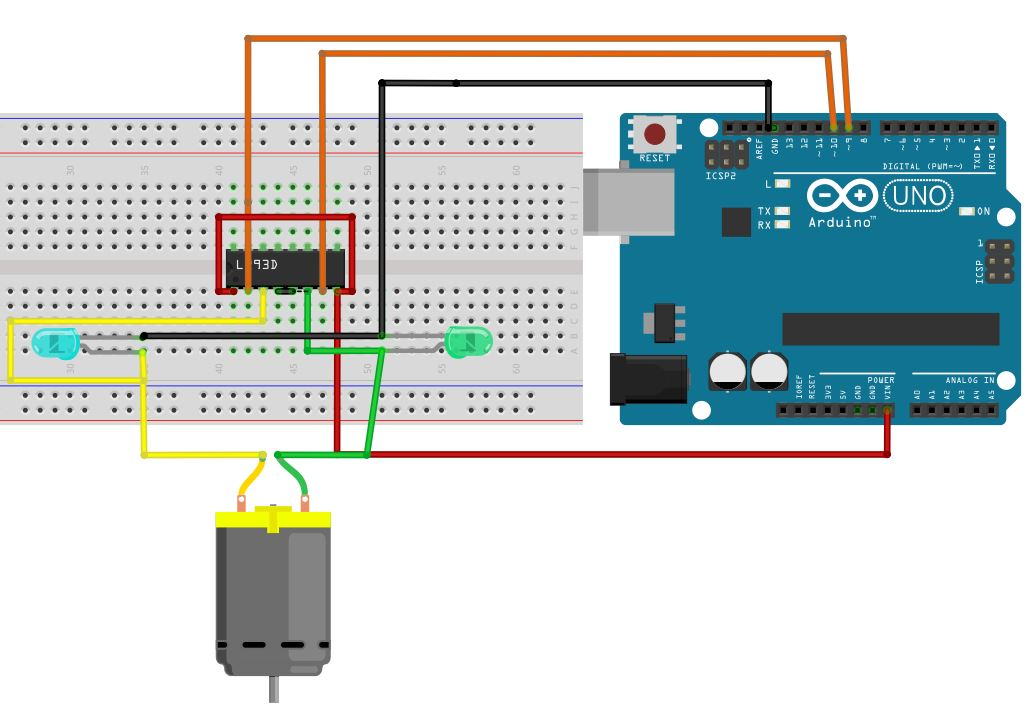
\includegraphics[width=1\textwidth]{billeder/Hardware/diagrammer/Motorbreadboard.JPG}
	\caption{Illustration af opstilling med motor(pumpe), motordriver og arduino}
	\label{fig:Motorbreadboard}
\end{figure}

For at teste motordriverens evne til at lave PWM med 12 volt, er PWM signalet fra Arduinoen og motordriveren sammenlignet med hinanden vha. et oscilloskop. Billeder fra denne test er vist på  billederne \ref{fig:25PWM}, \ref{fig:50PWM}, \ref{fig:75PWM} og \ref{fig:100PWM}. Den høje gule graf er fra motordriveren og den grønne lave graf er fra Arduinoen.

\newpage

 \begin{figure}[htbp] \centering
\begin{minipage}[b]{0.48\textwidth} \centering
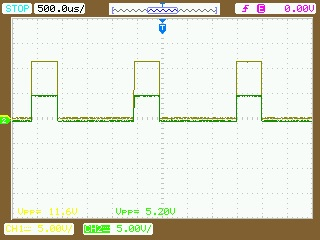
\includegraphics[width=1.00\textwidth]{billeder/Hardware/motor25PWM.jpg} % Left picture
\end{minipage} \hfill
\begin{minipage}[b]{0.48\textwidth} \centering
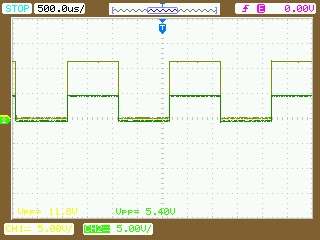
\includegraphics[width=1.00\textwidth]{billeder/Hardware/motor50PWM.jpg} % Right picture
\end{minipage} \\ % Captions og labels
\begin{minipage}[t]{0.48\textwidth}
\caption{Arduino og motordriver med 25$\%$ PWM} % Left caption and label
\label{fig:25PWM}
\end{minipage} \hfill
\begin{minipage}[t]{0.48\textwidth}
\caption{Arduino og motordriver med 50$\%$ PWM} % Right caption and label
\label{fig:50PWM}
\end{minipage}
\end{figure}

 \begin{figure}[htbp] \centering
\begin{minipage}[b]{0.48\textwidth} \centering
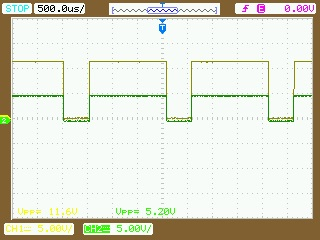
\includegraphics[width=1.00\textwidth]{billeder/Hardware/motor75PWM.jpg} % Left picture
\end{minipage} \hfill
\begin{minipage}[b]{0.48\textwidth} \centering
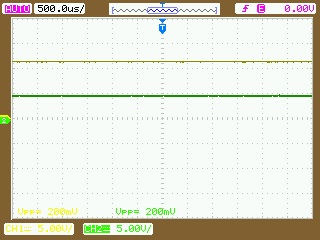
\includegraphics[width=1.00\textwidth]{billeder/Hardware/motor100PWM.jpg} % Right picture
\end{minipage} \\ % Captions og labels
\begin{minipage}[t]{0.48\textwidth}
\caption{Arduino og motordriver med 75$\%$ PWM} % Left caption and label
\label{fig:75PWM}
\end{minipage} \hfill
\begin{minipage}[t]{0.48\textwidth}
\caption{Arduino og motordriver med 100$\%$ PWM} % Right caption and label
\label{fig:100PWM}
\end{minipage}
\end{figure}

De elementære funktioner, som er brugt til test koden er \textit{digitalWrite(9, LOW);} og \textit{analogWrite(10, 127);}. Se hele testkoden i bilag \ref{bilag:TKpumpe}

\newpage

 \subsection{Ventil}
Ventilen skal sortere de langerhanske øer fra det eksokrine væv, derfor er ventilen en vigtig del af hardwaren. I integrationstesten bør tidsintervallet med hvornår ventilen skal åbnes og lukkes udføres, for en sikring af at øerne bliver isoleret.
\subsubsection{Enhedstest for ventil}
På figur \ref{fig:ventilbreadboard} er det illustreret hvordan testopstilling er sat op på et \textit{fumlebræt}. I test koden er der hovedsagligt brugt \textit{digitalWrite(8, LOW);} og \textit{digitalWrite(8, HIGH);}, hvorved Arduinoen sætter udgangen lav(0V) og høj(5V). Motordriveren bruger signalet til det at give ventilen 12V når den er høj. Se bilag \ref{bilag:TKventil} for hele testkoden.

\begin{figure}[H]
	\centering
	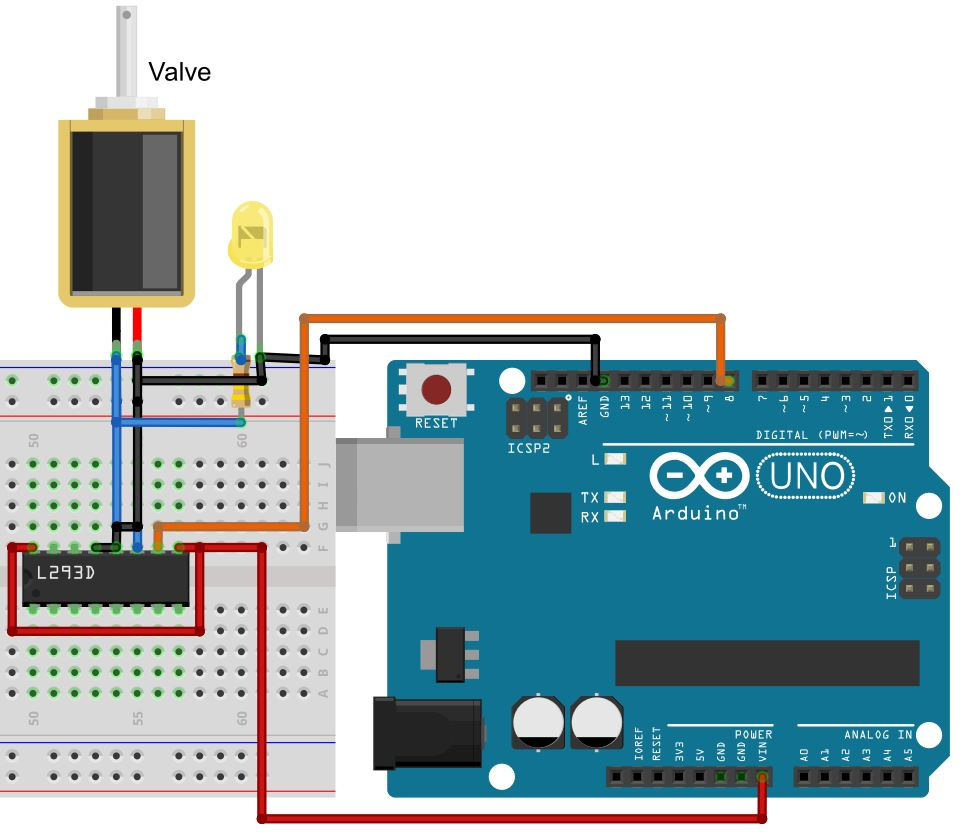
\includegraphics[width=1\textwidth]{billeder/Hardware/diagrammer/Ventilbreadboard.JPG}
	\caption{Illustration af testopstilling med ventil og motordriver}
	\label{fig:ventilbreadboard}
\end{figure} 
 
\newpage
 \subsection{Kameralys}
 \label{subsec:kameralys}
Kameralyset skal hjælpe operatøren med at optimere lysforholdet til kameraet for at maksimere forholdene og muligheden for at detektere de langerhanske øer. Testen burde være lavet med lysdioderne inde i kamerahuset, for at optimere feedbacket fra kameraet ved at ændre lysstyrken. Grundet kameraets manglende kvalitet er denne test nedprioriteret.

\subsubsection{Enhedstest for Kameralyset}
På figur \ref{fig:LEDbreadboard} vises testopstilling på et \textit{fumlebræt} for kameralyset er der brugt samme test kode som til pumpen se afsnit \ref{subsubsec:enhedstestmotor}. 

\begin{figure}[H]
	\centering
	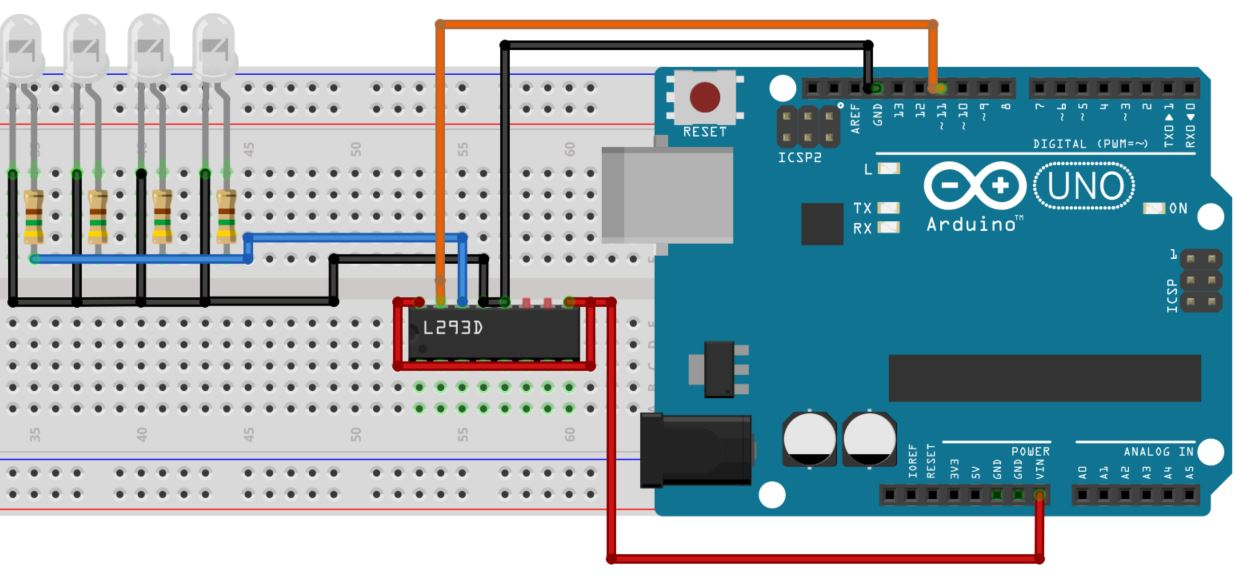
\includegraphics[width=1\textwidth]{billeder/Hardware/diagrammer/LEDbreadboard.JPG}
	\caption{Illustration af testopstilling med kameralys og motordriver}
	\label{fig:LEDbreadboard}
\end{figure}

 
\newpage 
\subsection{Ikke-elektroniske dele}
På figur \ref{fig:nonelectronic} vises en illustration af de ikke-elektroniske dele for hele systemet. De ikke-elektroniske dele består af en opløsningsningsbeholder, som navnet fortæller, indeholder opløsningen med de langerhanske øer. Fra opløsningsbeholder går en teflonslange, den er hård hvilket er en fordel når den skal suge væsken op. For at en peristaltisk pumpe kan benyttes skal det være en silikoneslange, da den er eftergivelig. Overgangen fra teflonslangen til slikoneslangen er oprettet vha. en slangeadapter. Derefter føres silikone slangen til pumpen, til ventilen, hvor fra der går en silikoneslange fra hver af ventilens studser. Silikoneslangerne fra ventilen føres videre til wastebeholderen og beholderen til de isoleret øer.

\begin{figure}[H]
	\centering
	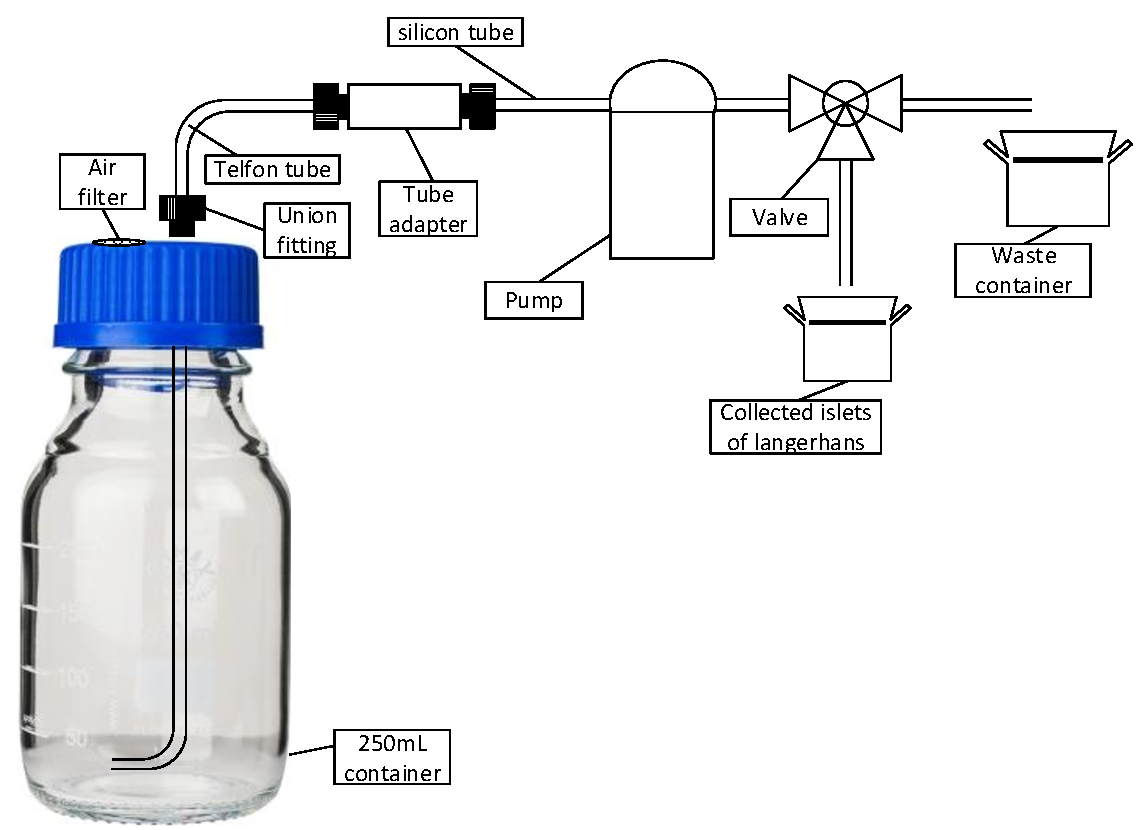
\includegraphics[width=1\textwidth]{billeder/Hardware/ikkeelektronisk.pdf}
	\caption{Illustration af ikke elektroniske dele}
	\label{fig:nonelectronic}
\end{figure}

Til test af ikke-elektroniske dele, er simuleringsvæsken med timianfrø og demineraliseret vand brugt. Timianfrøene der er brugt har en størrelse på 0.4mm hvilket burde kunne komme igennem, men frøene stopper ved ventilen. Derfor opfattes testen af ventilen som en fejlet test. Det bør undersøges hvorfor at frøene stopper ved ventilen, i datablad \ref{bilag:ventil} står der, at ventilens indgange er på 1mm. 

\newpage
\subsubsection{Stykliste} 
\begin{center}
		\begin{longtable}{ | m{6cm} | m{4cm}| m{2cm}| } 
			\hline
			\textbf{Beskrivelse} &\textbf{Type} & \textbf{Antal} \\ 
			\hline
			Opløsningsbeholder & ML 33184 & 1 stk \\ 
			\hline
			Flaskeadapter låg & ML 75441 & 1 stk \\ 
			\hline
			1/4" Prop til låg & UP P309 & 1 stk \\ 
			\hline
			1/16" Skrue flangeløs & UP P201 & 1 stk \\ 
			\hline
			1/16" Ferrule flangeløs & UP P200 & 1 stk \\ 
			\hline
			Flaskeadapter filter & n/a & 1 stk \\ 
			\hline	
			Teflonslange & ML 94142 & 0.2 m \\ 
			\hline
			Slangeadapter & UP P630 + UP646 & 1 stk \\ 
			\hline
			Silikoneslange(0.5mm) & n/a & 0.3 m \\ 
			\hline
			Slangestudser til ventil(10-32) & VP X210-60005 & 3stk \\ 
			\hline
		\end{longtable}
\end{center}

 
\subsection{PCB design} 
For at samle hardwaren i projektet er der lavet et printkort formet, som et shield til Arduino platformen. På printet er motordriveren der driver pumpen, ventilen og kameralyset. Motordriveren forsynes igennem en ekstern strømforsyning, som derved forsyner delene motordriveren styrer. I kredsløbet er der en operationsforstærker, som har til opgave at forstærke signalet fra vægtcellen og leverer det til ADC'en på Arduinoen. Pinheaderne på printet er med lange ben for, at de passer ned i Arduinoens pinheadere. Til at forbinde pumpen og ventilen, er der brugt stiktypen molex 5566-4 som kan trække en stor strøm. Til de to komponenter skal der kun bruges to ledninger, men for at sikre at stikkene ikke sættes forkert er der valgt et 4pin stik, hvor forbindelses benene er forskellige. Det betyder at hvis stikkene ved en fejl bliver ombyttet, vil hverken pumpen eller ventilen virke. Til kameralyset benyttes et 5 polet stik af typen molex 5268-05, stikket tåler en mindre strøm end de andre stik, men nok til kameralyset. Til vægtcellen er der valgt et stik af samme type, men i en 4 polet udgave. På printet er der lysindikatorer til at hjælpe med fejlfinding og service på systemet. Lysindikatorer består af 3 lysdioder; LED1 lyser når at ventilen er åben, LED2 lyser når motoren kører fremad og LED3 lyser, hvis motoren kører baglæns. Ydermere er der placeret kondensatorer parallelt med forsyningerne til at afkoble støj fra miljøet omkring systemet.

\newpage
\subsubsection{PCB kredsløbsdiagram}
På figur \ref{fig:PCBdiagram} er vist kredsløbet for printkortet i \textit{Eagle}. I diagrammet er der valgt at bruge GND symbolet i stedet for at forbinde signalerne til hinanden, dette er gjort for at simplificere diagrammet. JP er pinheaderne der forbinder signalet til arduinoen, stik er betegnet med X, C er kondensatorer og R er modstande.

\begin{figure}[H]

	\centering
	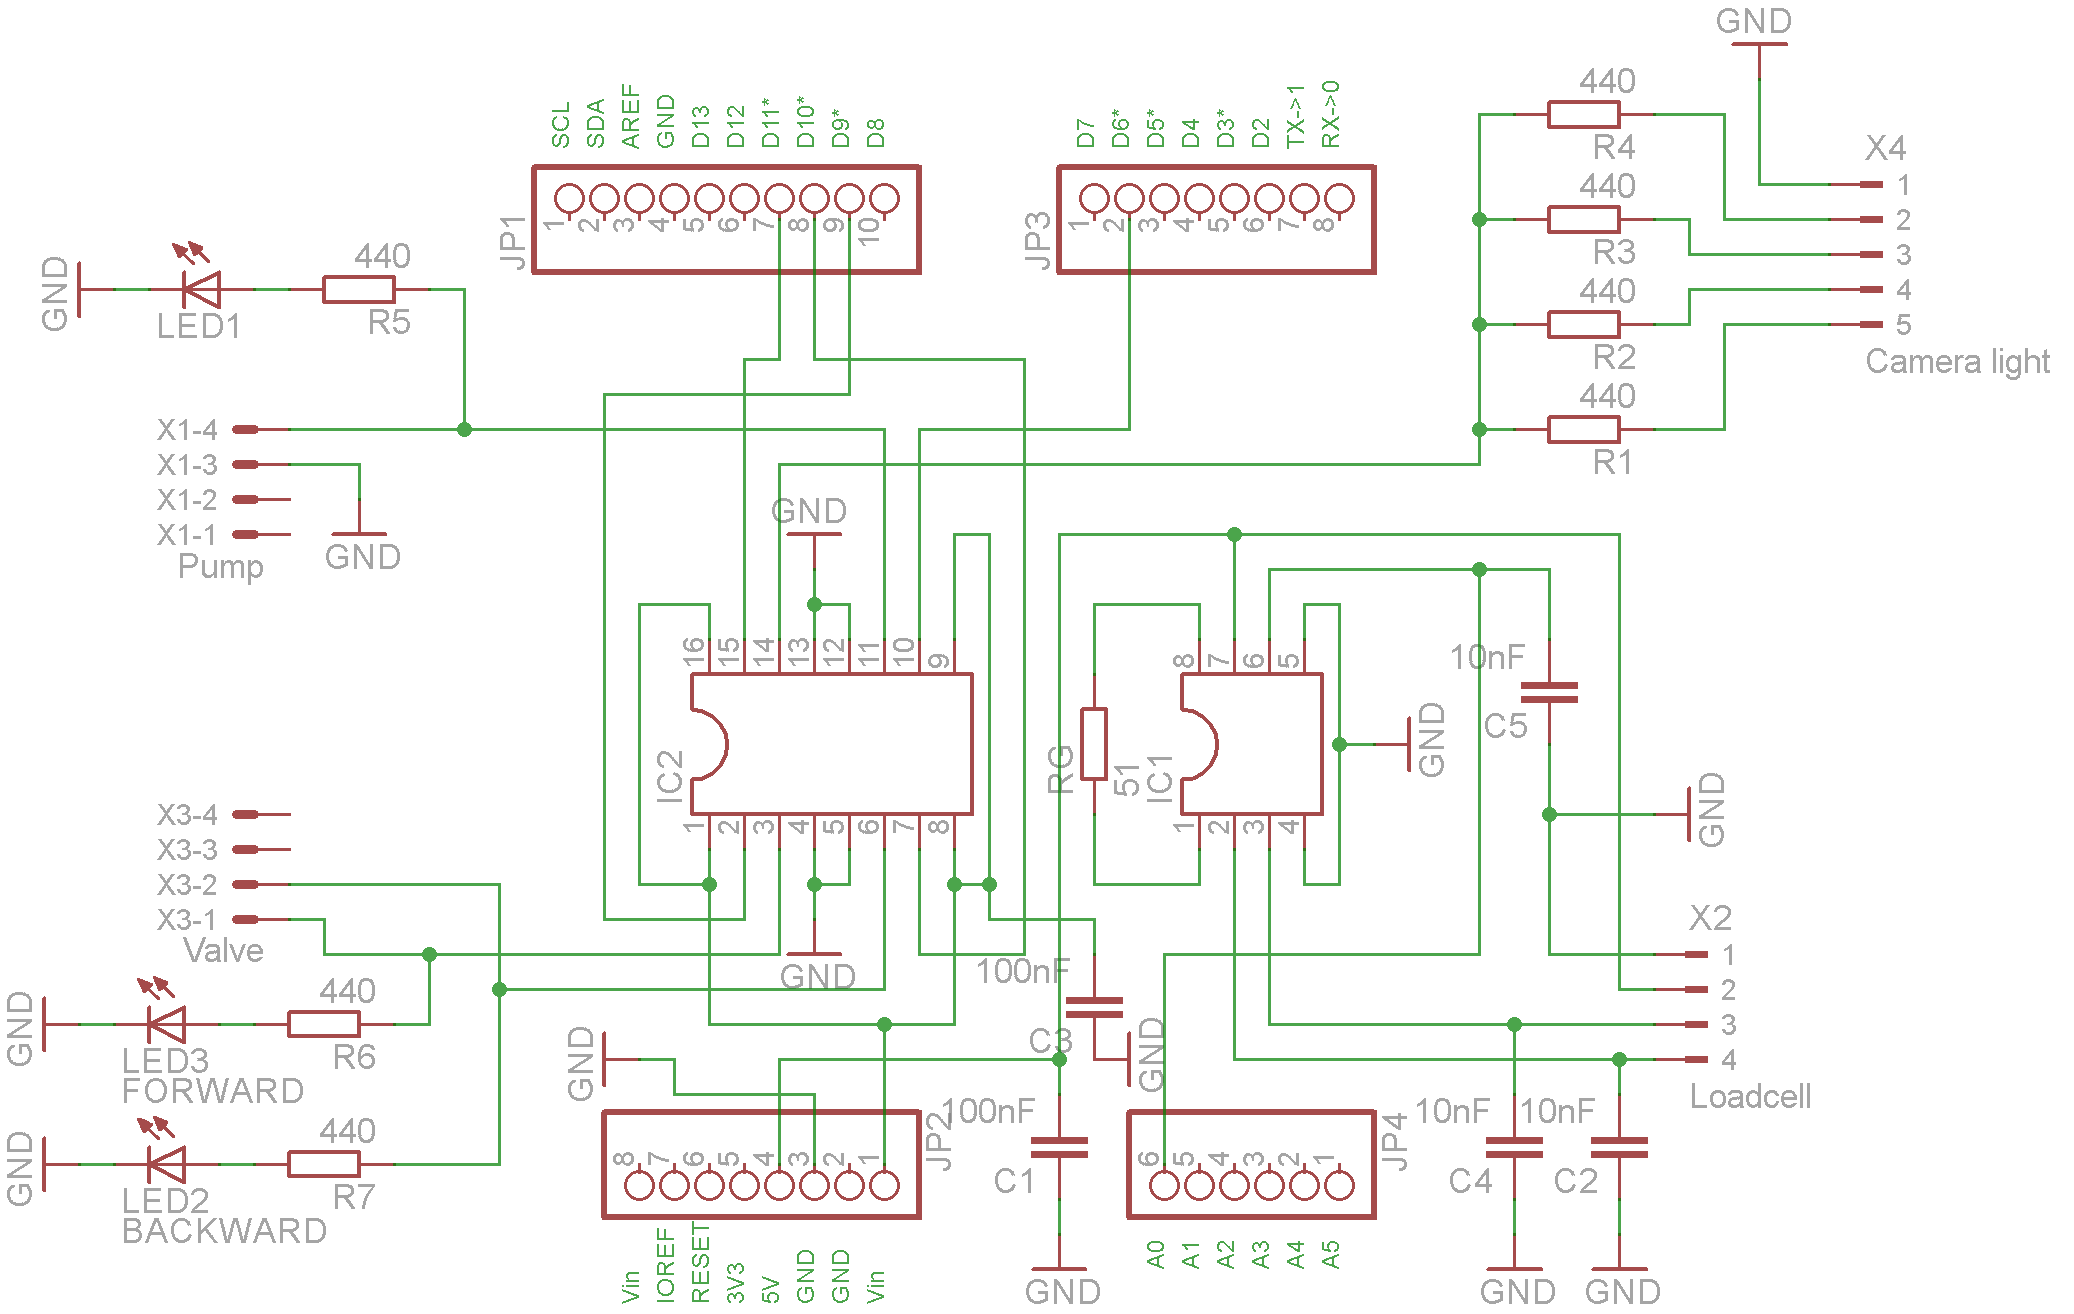
\includegraphics[width=1\textwidth]{billeder/hardware/Diagram.png}
	\caption{Diagram for printkortet}
	\label{fig:PCBdiagram}
\end{figure}

\newpage
\subsubsection{PCB toplayout}
På topplanet vist på \ref{fig:PCBtoplayout} er komponenterne til printet placeret. Der er forsøgt at lave de fleste forbindelser i dette plan for, at undgå brud i groundplanet. Silketrykket er ikke lavet, som vist på figur \ref{fig:PCBtoplayout} fordi det ikke laves på Ingeniørhøjskolens print produktion. Det er bl.a. derfor at alt den beskrivende tekst er lavet i top kobber laget. 

\begin{figure}[H]
	\centering
	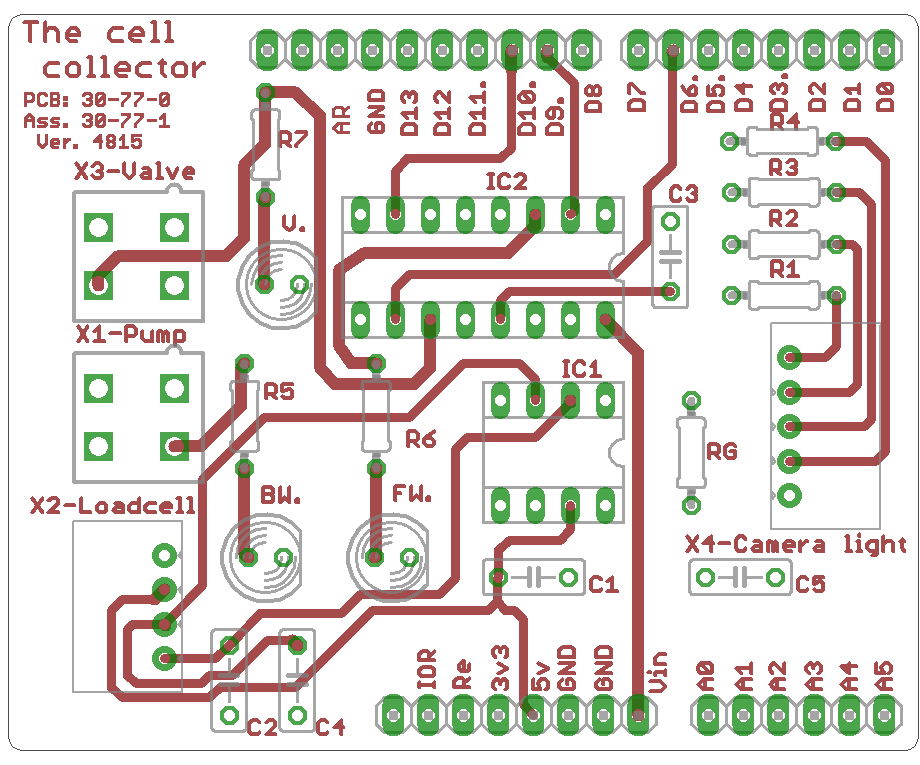
\includegraphics[width=1\textwidth]{billeder/hardware/Toplayout.png}
	\caption{PCB toplayout}
	\label{fig:PCBtoplayout}
\end{figure}

\newpage
\subsubsection{PCB bundlayout}
I bundlaget er der valgt at bruge et groundplan af følgende grunde; for at mindske indstrålingen af EMC, bruge den som køleplade til L293D og mindske fremførelsen af ground banerne. 

\begin{figure}[H]
	\centering
	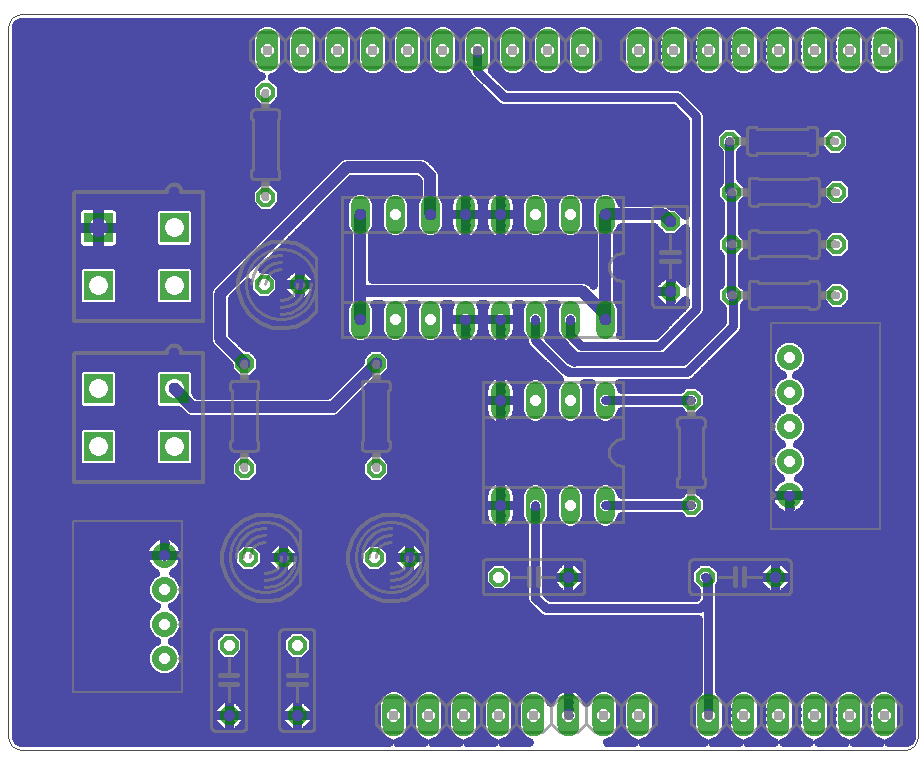
\includegraphics[width=1\textwidth]{billeder/hardware/Bundlayout.png}
	\caption{PCB bundlayout med groundplane}
	\label{fig:PCBbundlayout}
\end{figure}

\newpage
\subsubsection{Stykliste til PCB: 30-77-1}
Til samling af printet skal der bruges komponenterne i nedenstående tabel. 
\begin{center}
		\begin{longtable}{ | m{6cm} | m{4cm}| m{2cm}| } 
			\hline
			\textbf{Navn} &\textbf{Type} & \textbf{Antal} \\ 
			\hline
			C2,C4,C5 & 10nF & 3 stk \\ 
			\hline
			C1, C3 & 100nF & 2 stk \\ 
			\hline
			IC1 & INA114 & 1 stk \\ 
			\hline
			IC2 & L293D & 1 stk \\ 
			\hline
			Jp1-pinheader(stackable) & 1x10 & 1 stk \\ 
			\hline
			Jp2,3-pinheader(stackable) & 1x8 & 2 stk \\ 
			\hline
			Jp4-pinheader(stackable) & 1x6 & 1 stk \\ 
			\hline
			LED1-Green & 5mm(T13/4) & 1 stk \\ 
			\hline	
			LED2-Yellow & 5mm(T13/4) & 1 stk \\ 
			\hline
			LED3-Blue & 5mm(T13/4) & 1 stk \\ 
			\hline
			R1-R7 & 440$\Omega$ & 7 stk \\ 
			\hline
			RG & 51$\Omega$ & 1 stk \\ 
			\hline
			X1,X3 & molex 5566-4 & 2 stk \\ 
			\hline
			X2 & molex 5268-04 & 1 stk \\ 
			\hline
			X4 & molex 5268-05 & 1 stk \\ 
			\hline
		\end{longtable}
\end{center}

\subsubsection{Stykliste for stik til print}
For at sætte pumpe, ventil, vægtcelle og kameralyset til printkortet er komponenterne i nedenstående tabel nødvendige. 
\begin{center}
		\begin{longtable}{ | m{6cm} | m{4cm}| m{2cm}| } 
			\hline
			\textbf{Navn} &\textbf{Type} & \textbf{Antal} \\ 
			\hline
			X1,X3 & 2x2 Minifit Jr.(5557) & 2 stk \\ 
			\hline
			X1,X3 & Crimp(5556) & 4 stk \\ 
			\hline
			X2 & Polantal 4(5037) & 1 stk \\ 
			\hline
			X4 & Polantal 5(5037) & 1 stk \\ 
			\hline
			X2,X4 & Crimp(5263) & 9 stk \\ 
			\hline
		\end{longtable}
\end{center}

 